\section{Syntax}

\subsection{Text}

Display text in \textbf{bold}, \textit{italic}, \texttt{typewriter} \cite{overleaf_font}. Note that underscores within \enquote{\texttt{\textbackslash texttt\{\}}} require to be escaped like \enquote{\texttt{a\textbackslash\_b}}.

Embed website links with \href{https://www.overleaf.com/learn/latex/Hyperlinks}{displaying text}, \url{https://www.overleaf.com/learn/latex/Hyperlinks} \cite{overleaf_link}.

Use different formats of list to display \cite{overleaf_list}:
\begin{itemize}
    \item item 1
        \begin{enumerate}
            \item item 1
                \begin{description}
                    \item[Bold title] item 1
                \end{description}
        \end{enumerate}
\end{itemize}

Use special characters like \ding{52}, \ding{56} \cite{pifont}.

Embed code from file as figure, as shown in \Cref{fig:embed_ef,fig:embed_pf}.
\begin{figure}[H]
\lstinputlisting[
    language=Bash,
    showspaces=false,
    basicstyle=\ttfamily\footnotesize,
    numbers=left,
    numberstyle=\tiny,
    commentstyle=\color{gray},
]{../script/example.sh}
\caption{Embed entire script file.}
\label{fig:embed_ef}
\end{figure}
\begin{figure}[H]
\lstinputlisting[
    linerange={3-4},
    language=Bash,
    showspaces=false,
    basicstyle=\ttfamily\footnotesize,
    numbers=left,
    numberstyle=\tiny,
    commentstyle=\color{gray},
]{../script/example.sh}
\caption{Embed selected lines script file.}
\label{fig:embed_pf}
\end{figure}

\subsection{Figure}

Various tools can be use to create figures and are roughly classified as 1 (best) to 3 (worst) in \autoref{table:fig_tool}.

\begin{center}
    \captionof{table}{Assessment of different tools to create figures.}
    \label{table:fig_tool}
    \begin{tabular}{ c c c c c c }
        \toprule
        Tool & Time required & Ease of use & Adjustability & Image quality & Scripting \\
        \midrule
        Mermaid (PDF) \cite{mermaid} & 1 & 1 & 3 & 1 & 1 \\
        draw.io (PDF) \cite{drawio} & 2 & 1 & 2 & 1 & 3 \\
        GNU Plot (PDF) \cite{gnuplot} & 3 & 3 & 1 & 1 & 1 \\
        MS PowerPoint & 2 & 1 & 2 & 3 & 3 \\
        \LaTeX\ TikZ \cite{tikz} & 3 & 3 & 1 & 1 & 1 \\
        \bottomrule
    \end{tabular}
\end{center}

To embed a downloaded figure or figure created with external tools mentioned in \autoref{table:fig_tool}, the following format can be used for PNG, JPG and PDF (best quality) format \cite{inserting_img}.

\begin{figure}[H]
    \centering
    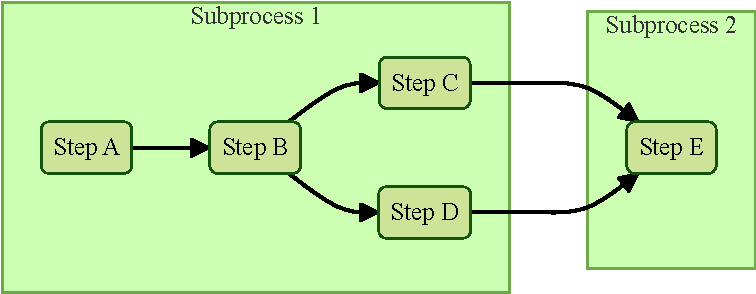
\includegraphics[width=0.8\textwidth]{../figure/mermaid_out/flowchart.pdf}
    \caption{A example of embedding a PDF image.}
    \label{fig:embed_pdf}
\end{figure}

To use TikZ in \LaTeX, visit the Minimal Working Example (MWE) example page \cite{tikz_example}. Additional packages will be needed and should be added in the \texttt{main.tex} file.

\subsection{Table}

A basic version of \LaTeX\ two by two table with custom border is shown in \autoref{table:tab1}; another table with specific column and row name is shown in \autoref{table:tab2}; an additional table with merged rows and columns is shown in \autoref{table:tab3}.

\begin{center}
    \captionof{table}{Basic table.}
    \label{table:tab1}
    \begin{tabular}{ c | c }
        \hline
        cell & cell \\
        cell & cell \\
        \hline
    \end{tabular}
\end{center}


\begin{center}
    \captionof{table}{Table with column and row names.}
    \label{table:tab2}
    \begin{tabular}{ c | c c }
        \toprule
         & Column A & Column B \\
        \midrule
        Row 1 & cell & cell \\
        Row 2 & cell & cell \\
        \bottomrule
    \end{tabular}
\end{center}

\begin{center}
    \captionof{table}{Table with merged rows and columns.}
    \label{table:tab3}
    \begin{tabular}{ c | c c }
        \toprule
         & Column A & Column B \\
        \midrule
        \multirow[t]{2}{*}{Row 1-2} & cell & cell \\
                                    & \multicolumn{2}{c}{merged cell} \\
        Row 3 & cell & cell \\
        \bottomrule
    \end{tabular}
\end{center}

If it is too confusing to edit the entire table manually, visit Table Generator for web-based Graphical User Interface (GUI) editor and copy the generated code into the document \cite{table_gen}.

\subsection{Equation}

When displaying math symbols, they can be used inline like $a+b=c$. As shwon in \autoref{eq:eq1}, it can be used to create complicated equations. It can use additional \enquote{aligned} environment to align multiple equations against certain location within equation with symbol $\&$, as shown in \autoref{eq:eq2}.

\begin{equation}
    a^2+b_1=\dfrac{\sum\limits^{m}_{n=1}c_n}{d}
    \label{eq:eq1}
\end{equation}

\begin{equation}
    \begin{aligned}
        a_1+b&=c \\
        \sqrt{d}&=c \\
        d&=\int^e_fx^5dx+\alpha^{2^2}
    \label{eq:eq2}
    \end{aligned}
\end{equation}

\subsection{Algorithm}

Algorithms can be expressed with basic usage of the \enquote{algorithm} environment, as shown in \autoref{alg:alg1}. If it requires math expressions, inline expression cna be mixed within, as shown in \autoref{alg:alg2} \cite{overleaf_alg}.

\begin{algorithm}
    \caption{Basic example of algorithm.}
    \label{alg:alg1}
    \begin{algorithmic}
        \If{condition A}
            \State state 1
        \Else
            \State state 2
        \EndIf
    \end{algorithmic}
\end{algorithm}

\begin{algorithm}
    \caption{Advance example of algorithm.}
    \label{alg:alg2}
    \begin{algorithmic}
        \If{$a+b+c>\text{threshold}$}
            \State $a+b+c$ is too large
        \Else
            \State Normal state
        \EndIf
    \end{algorithmic}
\end{algorithm}

\subsection{Citation}

When citing materials, the related information should be recorded in \textbf{BibTeX} format and stored in the file \enquote{\texttt{reference.bib}} which is specified by command \enquote{\texttt{\textbackslash\{bibliography reference\}}} in \enquote{\texttt{reference.tex}}.

Different categories of source can now be referenced in the document including \enquote{books}, \enquote{journals \& magazines}, and \enquote{conferences} \cite{10614682,10556316,9845195}. Their corresponding authors can be cited with \enquote{\citeauthor{10614682}}, \enquote{\citeauthor{10556316}}, \enquote{\citeauthor{9845195}}.

In some special cases, special symbols like \enquote{–} from ACM Digital Library in the \enquote{pages} field making the compiled result display pages with \enquote{p.} instead of \enquote{pp.} \cite{10.1145/3634737.3665024}. These special cases need to fix manually \cite{10.1145/3634737.3665024mod}.

\subsection{Custom commands and additional packages}
\label{sec_ccap}

% - single referencing - figure, table, eq, alg, section
The referencing to different sections within the document can be achieved with the following syntax: Fig. \ref{fig:embed_ef}, Table \ref{table:fig_tool}, \ref{eq:eq1} (equation), Algorithm \ref{alg:alg1}, Section \ref{sec_ccap}.

% - autoref
However, typing every single prefix of references is troublesome and error-prone. Another default syntax \enquote{\texttt{\textbackslash autoref}} can be used to achieve the same effect: \autoref{fig:embed_ef}, \autoref{table:fig_tool}, \autoref{eq:eq1} (equation), \autoref{alg:alg1}, \autoref{sec_ccap}. This requires the changes of \enquote{\texttt{autorefname}} in \texttt{main.tex}, and have the downside of unable to combine multiple references together.

% - cref - multi-reference syntax
To overcome the downside of \enquote{\texttt{\textbackslash autoref}}, \enquote{\texttt{\textbackslash Cref}} can be used instead: \Cref{fig:embed_ef,fig:embed_pf,table:fig_tool,fig:embed_pdf,table:tab1,table:tab2,table:tab3,eq:eq1,eq:eq2,alg:alg1,alg:alg2}. Note that escaping underscores used in \enquote{\texttt{\textbackslash Cref}} like \enquote{\texttt{\textbackslash\_}} will result in error.

% - renew reference name (Fig. Tab. Eq. Alg.)
For both \enquote{\texttt{\textbackslash autoref}} and \enquote{\texttt{\textbackslash Cref}}, their automatically added prefix can be adjusted with \enquote{\texttt{autorefname}} and \enquote{\texttt{\textbackslash crefname}} correspondingly, and are configured in \texttt{main.tex}.

% - keywords, keywordscn
Keywords for both English (\enquote{\texttt{\textbackslash keywords}}) and Chinese (\enquote{\texttt{\textbackslash keywordscn}}) can be achieved with the special commands set in \texttt{main.tex}. Example of these are shown in \texttt{abstract\_English.tex} and \texttt{abstract\_Chinese.tex}.

% - add additional layer: paragraph
The default layer of section are \enquote{\textbackslash section}, \enquote{\textbackslash subsection}, \enquote{\textbackslash subsubsection}, and \enquote{\textbackslash paragraph}. \enquote{\textbackslash paragraph} is modified in this template to fit and number correctly.

% - enquote
% - nth
% - xurl

Additional package \enquote{csquotes} is used for the \enquote{\texttt{\textbackslash enquote}} command (\enquote{quotes}). Package \enquote{nth} is used for the \enquote{\texttt{\textbackslash nth}} command (\nth{5}). Package \enquote{xurl} is used so that command \enquote{\texttt{\textbackslash href\{\}\{\}}} and \enquote{\texttt{\textbackslash url\{\}}} still can have line wrap (\url{https://this.is.a.super.long.link.that.does.not.link.to.anything.but.to.trigger.line.wrap}).


\clearpage
